\chapter{Исследовательский раздел}

В данном разделе будут приведены примеры работы программы, постановка эксперимента.

\section{Демонстрация работы программы}

На рисунке \ref{fig:democonsole} представлен результат работы программы. Словарь состоит из 6438 пар ключ-значение, он считывается программой из csv-файла. Пользователь вводит вопрос на ограниченном естественном языке. Программа сначала выделяет объект, признак, терм, затем формирует и выводит ответ на основании выделенного из входного вопроса терма. Ответ представлен как <<название видео>> <<количество просмотров>>.


\captionsetup{justification=centering, singlelinecheck=false}
\begin{figure}[H]
	\centering
	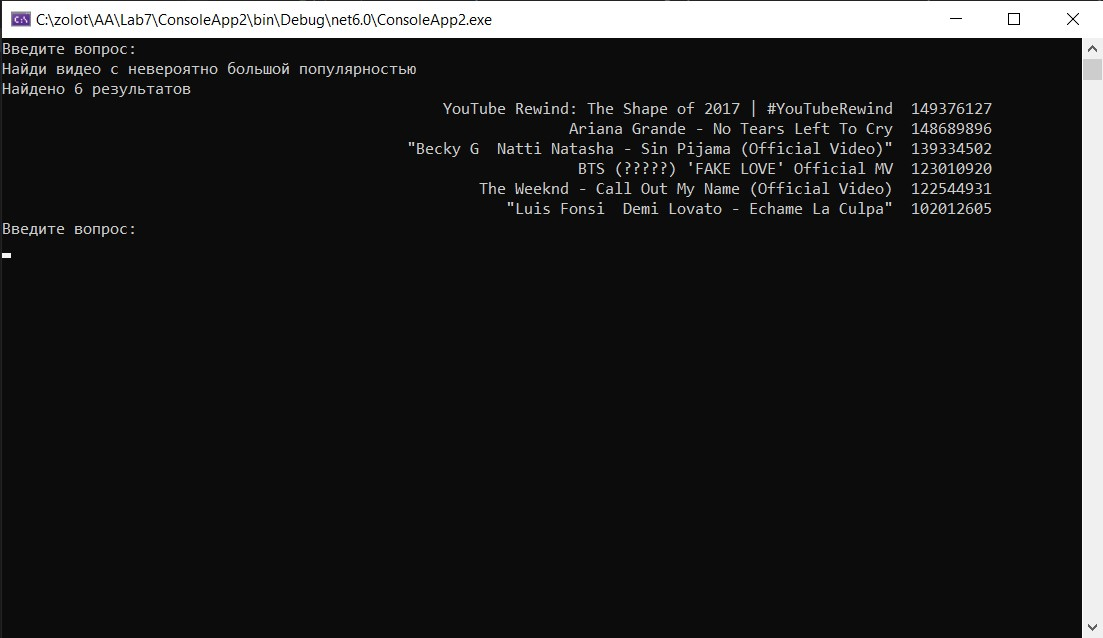
\includegraphics[width=1\linewidth]{inc/img/democonsole}
	\caption{Демонстрация работы программы}
	\label{fig:democonsole}
\end{figure}

\section{Выполнение эксперимента}

Для анкетирования респондентов была составлена таблица~\ref{tbl:anketa}, термы и значения представлены в \eqref{eq:term} и \eqref{eq:znach} соответственно.

\captionsetup{justification=raggedright,singlelinecheck=false}
\begin{table}[H]
	\begin{threeparttable}
		\caption{\label{tbl:anketa}Анкета респондентов}
		\begin{tabular}{|c|c|c|c|c|c|c|c|c|c|c|}
			\hline
			& \multicolumn{10}{c|}{Число просмотров видео на YouTube}\\\cline{2-11}
			Терм & 0&	10&	50&	100&	200&	500&	1 &	10 &	100 &	200\\
			& &	тыс&	тыс&	тыс&	тыс&тыс&млн &	млн &	млн& млн\\\hline
			очень маленькая	&&&&&&&&&&\\\hline
			не очень 	&&&&&&&&&&\\
			маленькая&&&&&&&&&&\\\hline
			маленькая	&&&&&&&&&&\\\hline
			небольшая	&&&&&&&&&&\\\hline
			средняя	&&&&&&&&&&\\\hline
			немаленькая	&&&&&&&&&&\\\hline
			не очень большая	&&&&&&&&&&\\\hline
			большая		&&&&&&&&&&\\\hline
			очень большая		&&&&&&&&&&\\\hline
		\end{tabular}
	\end{threeparttable}
\end{table} 

Для составления экспертной оценки были опрошены следующие студенты:
\begin{itemize}[label=---]
	\item Арсений Хрюкин;
	\item Дарья Татаринова;
	\item Чепиго Дарья;
	\item Николаев Сергей;
	\item Золотухин Алексей.
\end{itemize}

По итогам опроса получилась сводная таблица~\ref{tbl:exp} значений функции~\eqref{eq:mu}, графики этой функции для каждого терма представлены на рисунке~\ref{fig:exp}. В таблице~\ref{tbl:interval} представлены диапазоны значений числа просмотров, соответствующие термам. 

\captionsetup{justification=raggedright,singlelinecheck=false}
\begin{table}[H]
	\begin{threeparttable}
		\caption{\label{tbl:exp}Сводная таблица результатов анкетирования --- значения функций принадлежности $\mu_i(x_j)$ числа просмотров $x_j$ термам $t_i$}
		\begin{tabular}{|c|c|c|c|c|c|c|c|c|c|c|}
			\hline
			& \multicolumn{10}{c|}{Число просмотров видео на YouTube ---$x_j$}\\\cline{2-11}
			Терм $t_i$ & 0&	10&	50&	100&	200&	500&	1 &	10 &	100 &	200\\
			& &	тыс&	тыс&	тыс&	тыс&тыс&млн &	млн &	млн& млн\\\hline
			очень &&&&&&&&&&\\
маленькая	&	0,8	&	0,2	&	0	&	0	&	0	&	0	&	0	&	0	&	0	&	0	\\\hline
не очень&&&&&&&&&&\\
 маленькая	&	0,4	&	0,6	&	0	&	0	&	0	&	0	&	0	&	0	&	0	&	0	\\\hline&&&&&&&&&&\\
маленькая	&	0	&	0,4	&	0,6	&	0	&	0	&	0	&	0	&	0	&	0	&	0	\\\hline&&&&&&&&&&\\
небольшая	&	0	&	0,6	&	0,4	&	0,4	&	0,4	&	0,2	&	0	&	0	&	0	&	0	\\\hline&&&&&&&&&&\\
средняя	&	0	&	0	&	0,4	&	0,4	&	0	&	0,2	&	0,2	&	0	&	0	&	0	\\\hline&&&&&&&&&&\\
немаленькая	&	0	&	0	&	0,2	&	0,4	&	0,6	&	0	&	0	&	0	&	0	&	0	\\\hline не очень &&&&&&&&&&\\
 большая	&	0	&	0	&	0	&	0	&	0,2	&	0,6	&	0,2	&	0	&	0	&	0	\\\hline&&&&&&&&&&\\
большая	&	0	&	0	&	0	&	0	&	0	&	0,2	&	0,6	&	0,6	&	0	&	0	\\\hline&&&&&&&&&&\\
очень большая	&	0	&	0	&	0	&	0	&	0	&	0	&	0	&	0,6	&	0,6	&	0,2	\\\hline невероятно&&&&&&&&&&\\
 большая	&	0	&	0	&	0	&	0	&	0	&	0	&	0	&	0	&	0,6	&	1	\\\hline
		\end{tabular}
	\end{threeparttable}
\end{table} 

\captionsetup{justification=centering,singlelinecheck=false}
\begin{figure}[H]
	\centering
	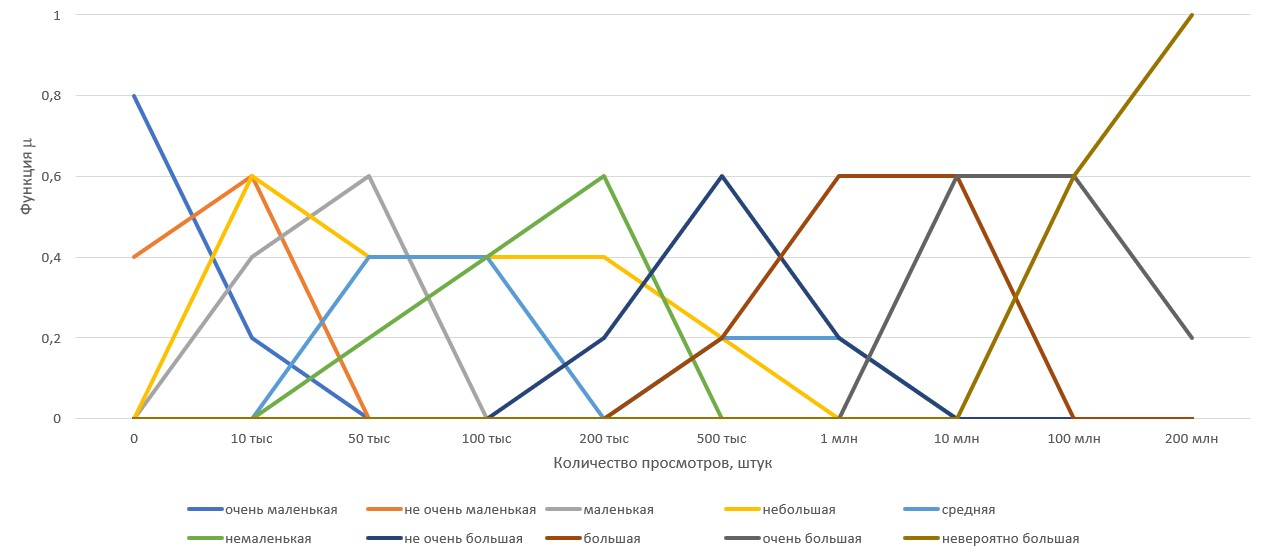
\includegraphics[width=1\linewidth]{inc/img/time}
	\caption{Графики функций $\mu_i(x_j)$ }
	\label{fig:exp}
\end{figure}

\captionsetup{justification=raggedright,singlelinecheck=false}
\begin{table}[H]
	\begin{center}
		\begin{threeparttable}
		\caption{\label{tbl:interval}Сопоставленные с лингвистической переменной диапазоны значений числа просмотров}
		\begin{tabular}{|c|c|c|}
			\hline
			Значение переменной & Нижняя граница& Верхняя граница\\\hline
			очень маленькая	&	0	&	5 тыс	\\\hline
			не очень маленькая	&	5 тыс	&	10 тыс	\\\hline
			небольшая	&	10 тыс	&	30 тыс	\\\hline
			маленькая	&	30 тыс	&	66,67 тыс	\\\hline
			средняя	&	66,67 тыс	&	100 тыс	\\\hline
			немаленькая	&	100 тыс	&	320 тыс	\\\hline
			не очень большая	&	320 тыс	&	750 тыс	\\\hline
			большая	&	750 тыс	&	10 млн	\\\hline
			очень большая	&	10 млн	&	100 млн	\\\hline
			невероятно большая	&	100 млн 	&	200 млн	\\\hline
			
		\end{tabular}
	\end{threeparttable}
	\end{center}
\end{table} 

Уникальные вопросы, заданные респондентами следующие.
\begin{enumerate}
	\item Какие видео имеют большое количество просмотров?
	\item Найди видео с немаленьким числом просмотров.
	\item Какие видео посмотрело маленькое количество людей?
	\item Найди видео с невероятно большой популярностью.
	\item Покажи очень дорогие квартиры. 
	\item Какие студенты долго делают отчет по АА?
	\item Популярные видео.
\end{enumerate}

На рисунках \ref{fig:q1}, \ref{fig:q2}, \ref{fig:q3}, \ref{fig:q4}, \ref{fig:q5}, \ref{fig:q6}, \ref{fig:q7} представлены ответы на соответствующие вопросы.
\captionsetup{justification=centering,singlelinecheck=false}
\begin{figure}[H]
	\centering
	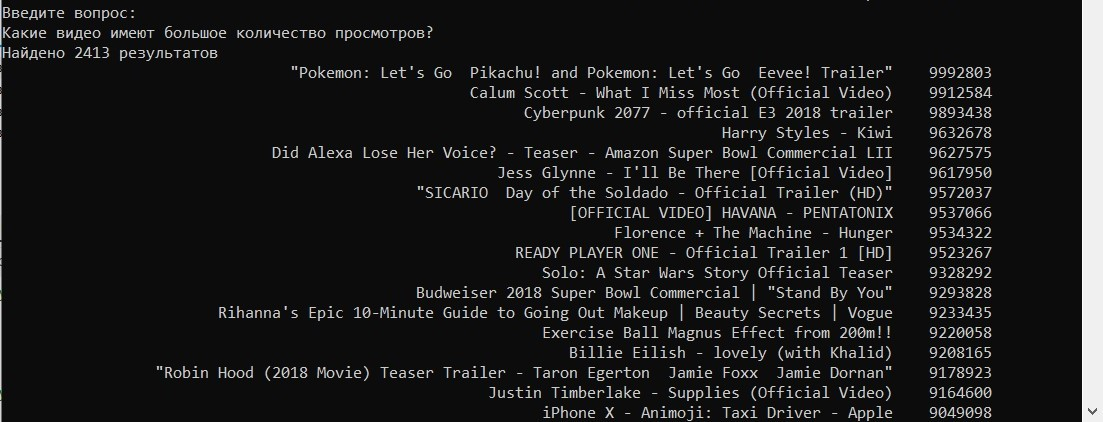
\includegraphics[width=1\linewidth]{inc/img/q1}
	\caption{Ответ на вопрос 1}
	\label{fig:q1}
\end{figure}
\begin{figure}[H]
	\centering
	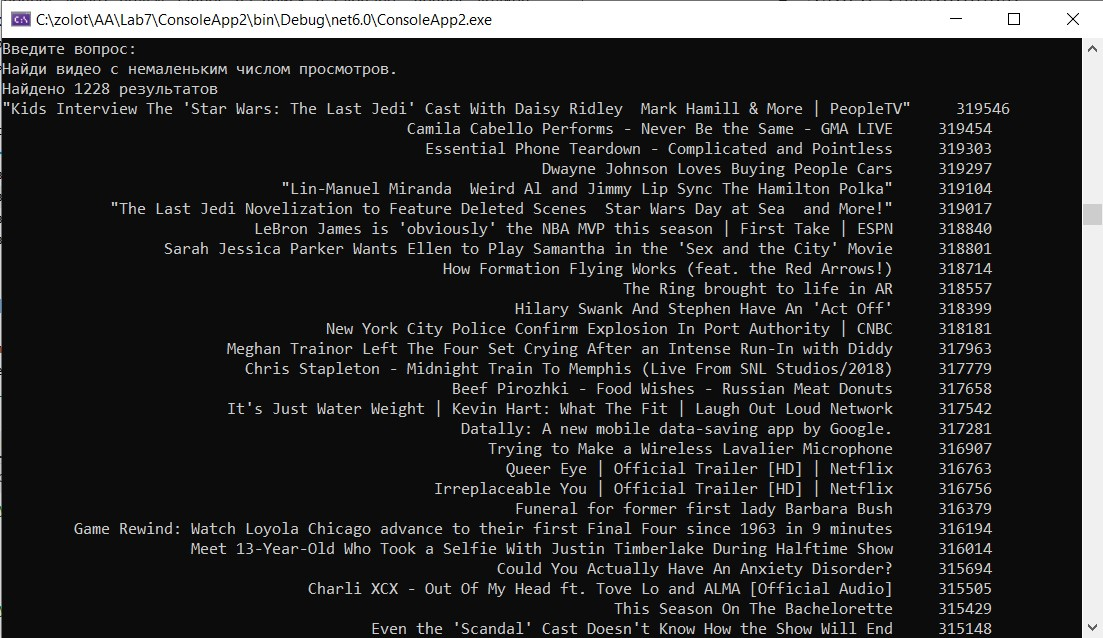
\includegraphics[width=1\linewidth]{inc/img/q2}
	\caption{Ответ на вопрос 2}
	\label{fig:q2}
\end{figure}
\begin{figure}[H]
	\centering
	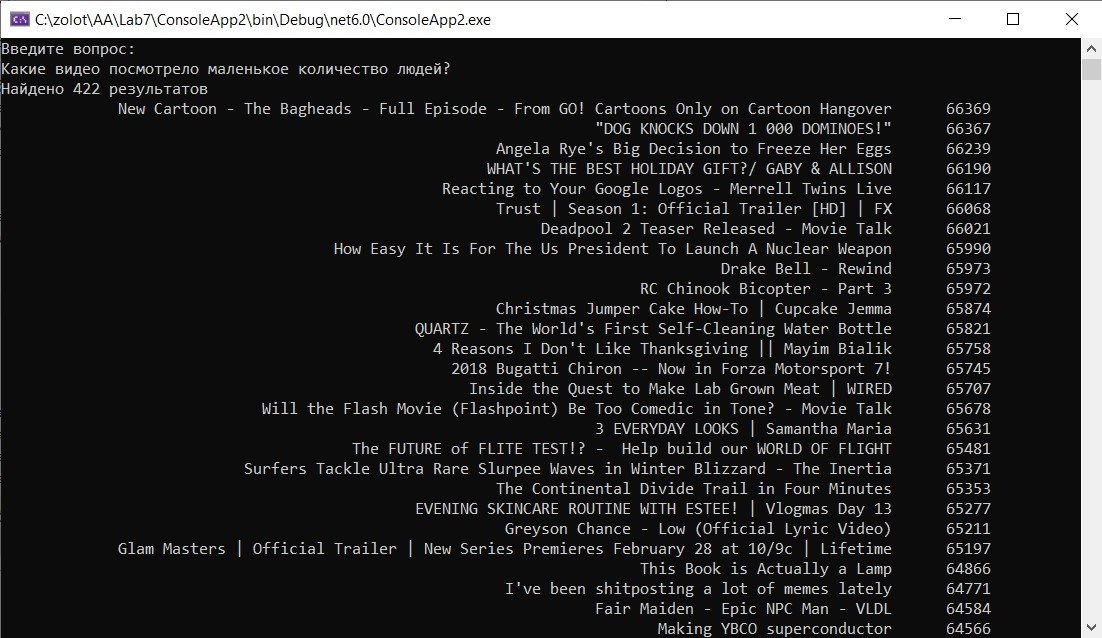
\includegraphics[width=1\linewidth]{inc/img/q3}
	\caption{Ответ на вопрос 3}
	\label{fig:q3}
\end{figure}
\begin{figure}[H]
	\centering
	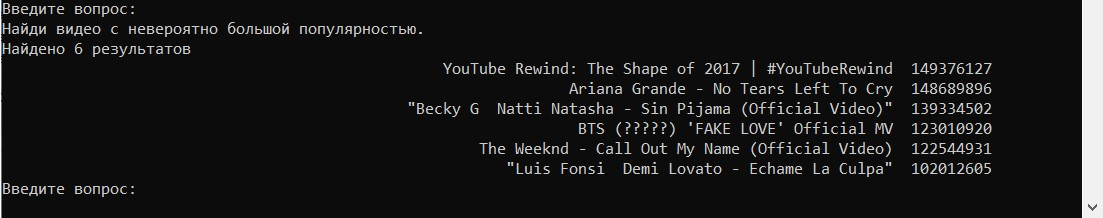
\includegraphics[width=1\linewidth]{inc/img/q4}
	\caption{Ответ на вопрос 4}
	\label{fig:q4}
\end{figure}
\begin{figure}[H]
	\centering
	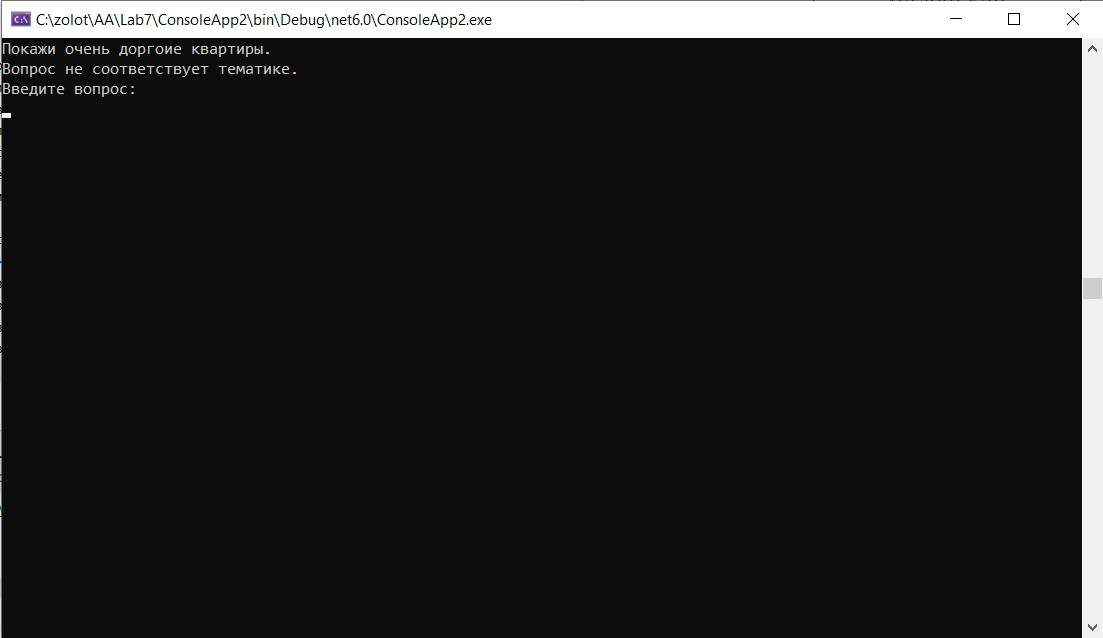
\includegraphics[width=1\linewidth]{inc/img/q5}
	\caption{Ответ на вопрос 5}
	\label{fig:q5}
\end{figure}
\begin{figure}[H]
	\centering
	
\includegraphics[width=0.5\linewidth]{inc/img/q6}
	\caption{Ответ на вопрос 6}
	\label{fig:q6}
\end{figure}
\begin{figure}[H]
	\centering
	
\includegraphics[width=0.3\linewidth]{inc/img/q7}
	\caption{Ответ на вопрос 7}
	\label{fig:q7}
\end{figure}
\section{Вывод}

По результатам экспертной оценки разработанная программа, реализующая предложенный метод поиска в словаре, отвечает исправно на заданные вопросы. Данная система в теории может применяться для автоматической выборки из словаря по запросам на ограниченном естественном языке.